\documentclass{beamer}
\usepackage{graphicx,amsmath,amsfonts,amssymb,listings,tikz}
\usepackage{multimedia}
\usetheme{Montpellier}
\usecolortheme{beaver}
\beamerdefaultoverlayspecification{<+->}
\definecolor{mygray}{rgb}{0.92,0.92,0.92}

\begin{document}

\section{Introduction}
\title{Harten's Multiresolution Scheme on Adaptive Mesh Refinement Blocks for More Efficient Simulation of Reactive Flows}
\author{Brandon Gusto} %
\institute{Dept. of Scientific Computing \\ Florida State University}
\date{\today}
\frame{\titlepage}

\section{Introduction}

\begin{frame}{Introduction}
    Many engineering applications depend on numerically solving systems of conservation laws of the form
    \begin{equation*}
        \mathbf{U}_{t} + \mathbf{F}(\mathbf{U})_{x} = \mathbf{S}(\mathbf{U})
    \end{equation*}
    where $\mathbf{U} = (\rho,\rho u,E)$ is a vector of conserved quantities,
    $\mathbf{F}(\mathbf{U})$ is a flux vector, and $\mathbf{S}(\mathbf{U})$ is a
    vector of source terms. The discretized solution is represented as
    averages over each cell
    \begin{equation*}
        \mathbf{U}_{i} = \frac{1}{|V_{i}|} \int_{V_{i}} \mathbf{U} dV.
    \end{equation*}
    where the $i$ denotes spatial index.
\end{frame}

\begin{frame}{Discretization}
    The semi-discretized form of the system of PDEs is
    \begin{equation*}
        \frac{\partial \mathbf{U}_{i}}{\partial t} = -\frac{1}{|V_{i}|} \left( \mathbf{F}_{i+\frac{1}{2}}
            - \mathbf{F}_{i-\frac{1}{2}} \right) + \mathbf{S}_{i}
    \end{equation*}
    where the source terms are also averaged over each cell
    \begin{equation*}
        \mathbf{S}_{i} = \frac{1}{|V_{i}|} \int_{V_{i}} \mathbf{S} dV.
    \end{equation*}

\end{frame}

\begin{frame}{Solution Approaches}
    These equations are typically solved on a Cartesian grid with non-uniform mesh spacing:
    \begin{itemize}
        \item<2-> the refinement is generally associated with localized features
        \item<3-> some type of estimator of the local error is needed
        \item<4-> typically a collection of cells (a block) is refined for efficiency
        \item<5-> blocks introduce inherent ``overresolution" in some regions of the mesh
    \end{itemize}
\end{frame}

\section{Refinement}

\begin{frame}{Block-Structured AMR}
    \begin{figure}
        \center
        \includegraphics[scale=0.4]{amr1.png}
    \end{figure}
\end{frame}

\begin{frame}{Block-Structured AMR}
    \begin{figure}
        \center
        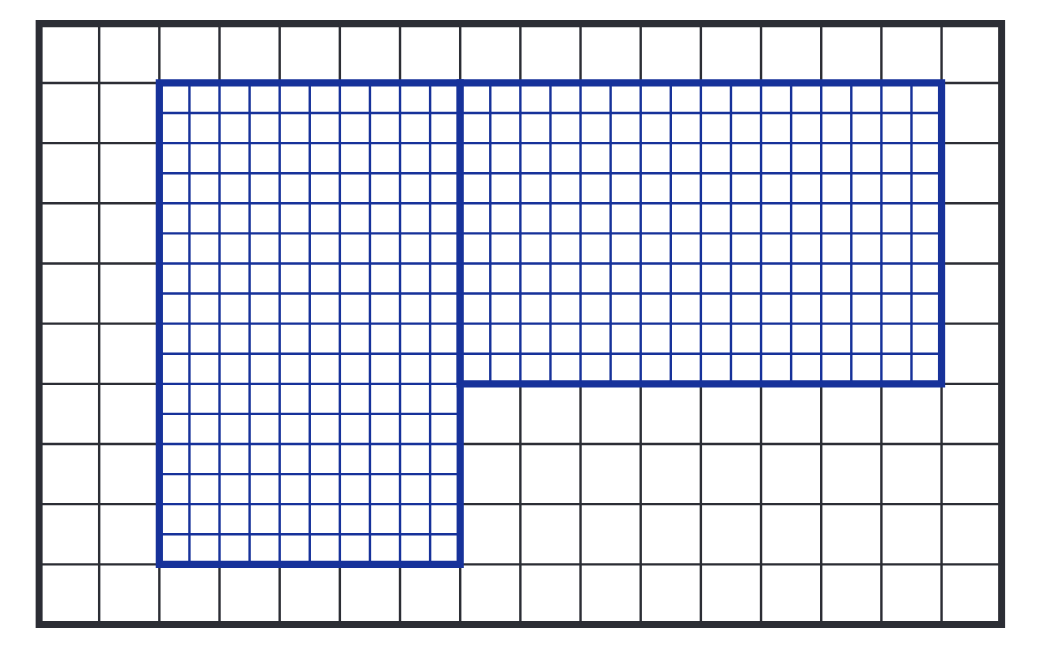
\includegraphics[scale=0.4]{amr2.png}
    \end{figure}
\end{frame}

\begin{frame}{Block-Structured AMR}
    \begin{figure}
        \center
        \includegraphics[scale=0.4]{amr3.png}
    \end{figure}
\end{frame}

\begin{frame}{Block-Structured AMR}
    \begin{figure}
        \center
        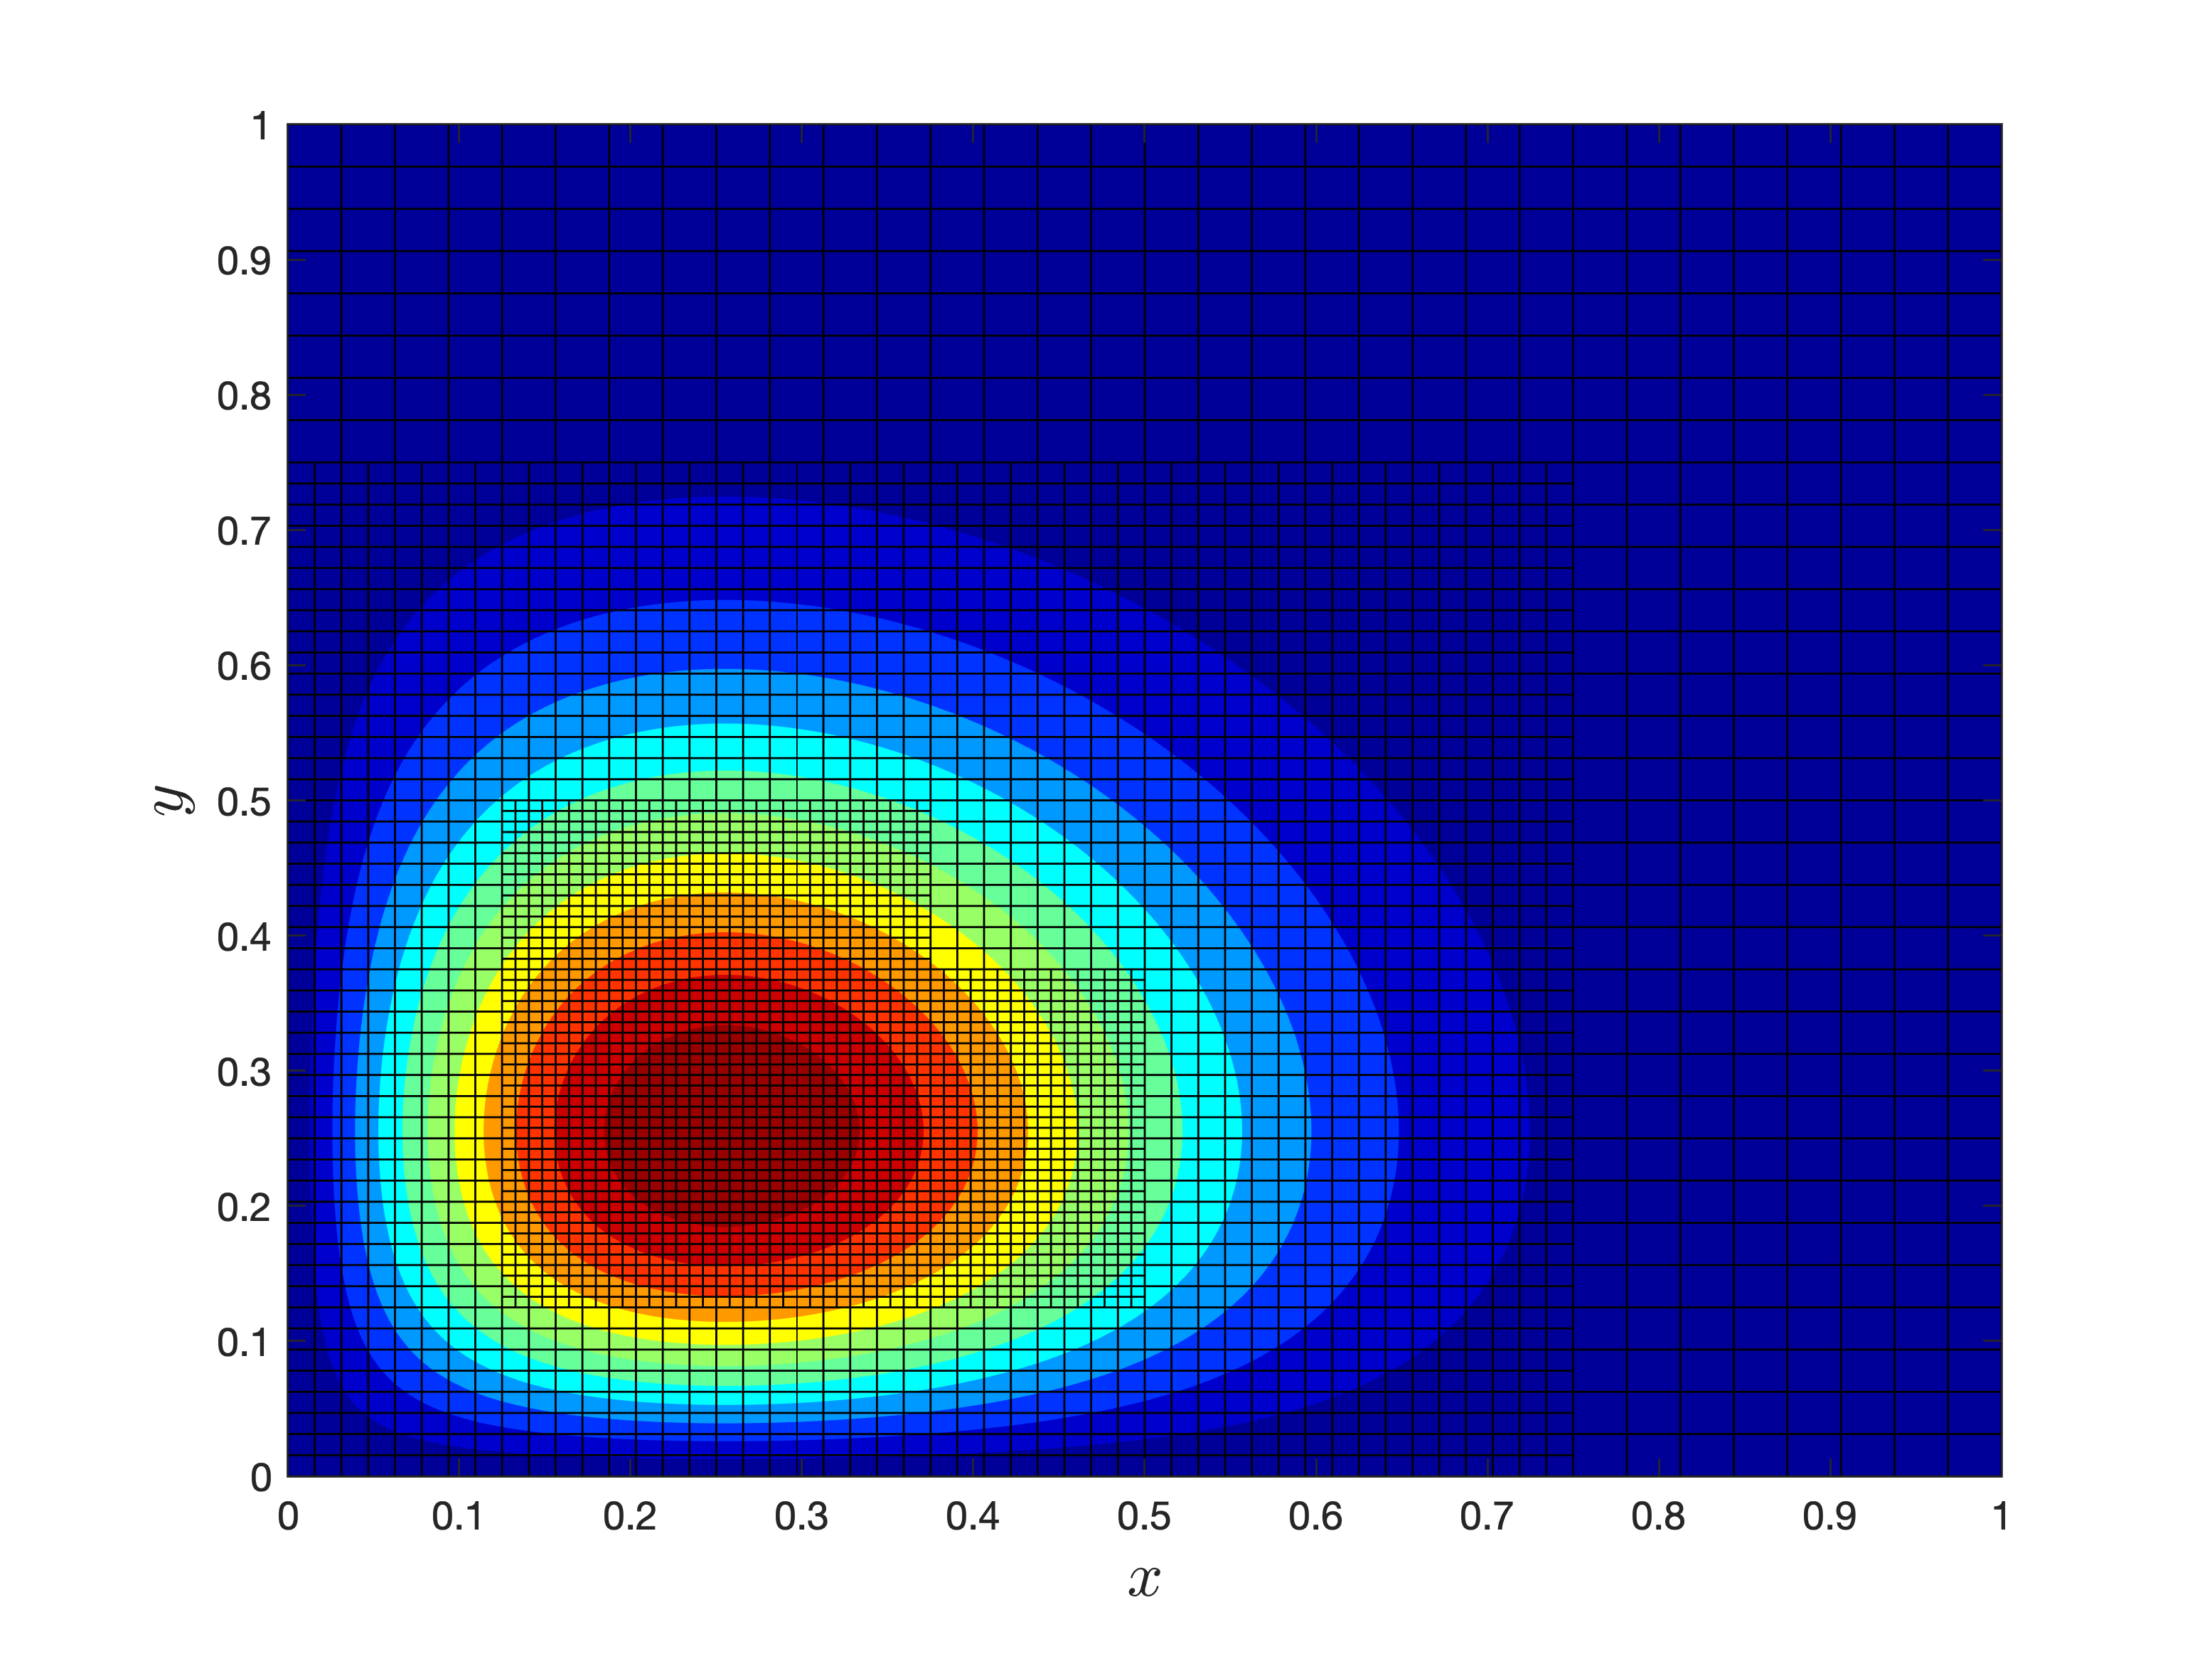
\includegraphics[scale=0.4]{amr4.png}
    \end{figure}
\end{frame}

\begin{frame}{Filling Factor}
    The filling factor is the number of cells in a block which were flagged, divided by the total.
    \begin{itemize}
        \item<2-> blocks with multiple parents becomes complicated
        \item<3-> communication between neighboring blocks becomes costly
    \end{itemize}
    \begin{figure}
        \center
        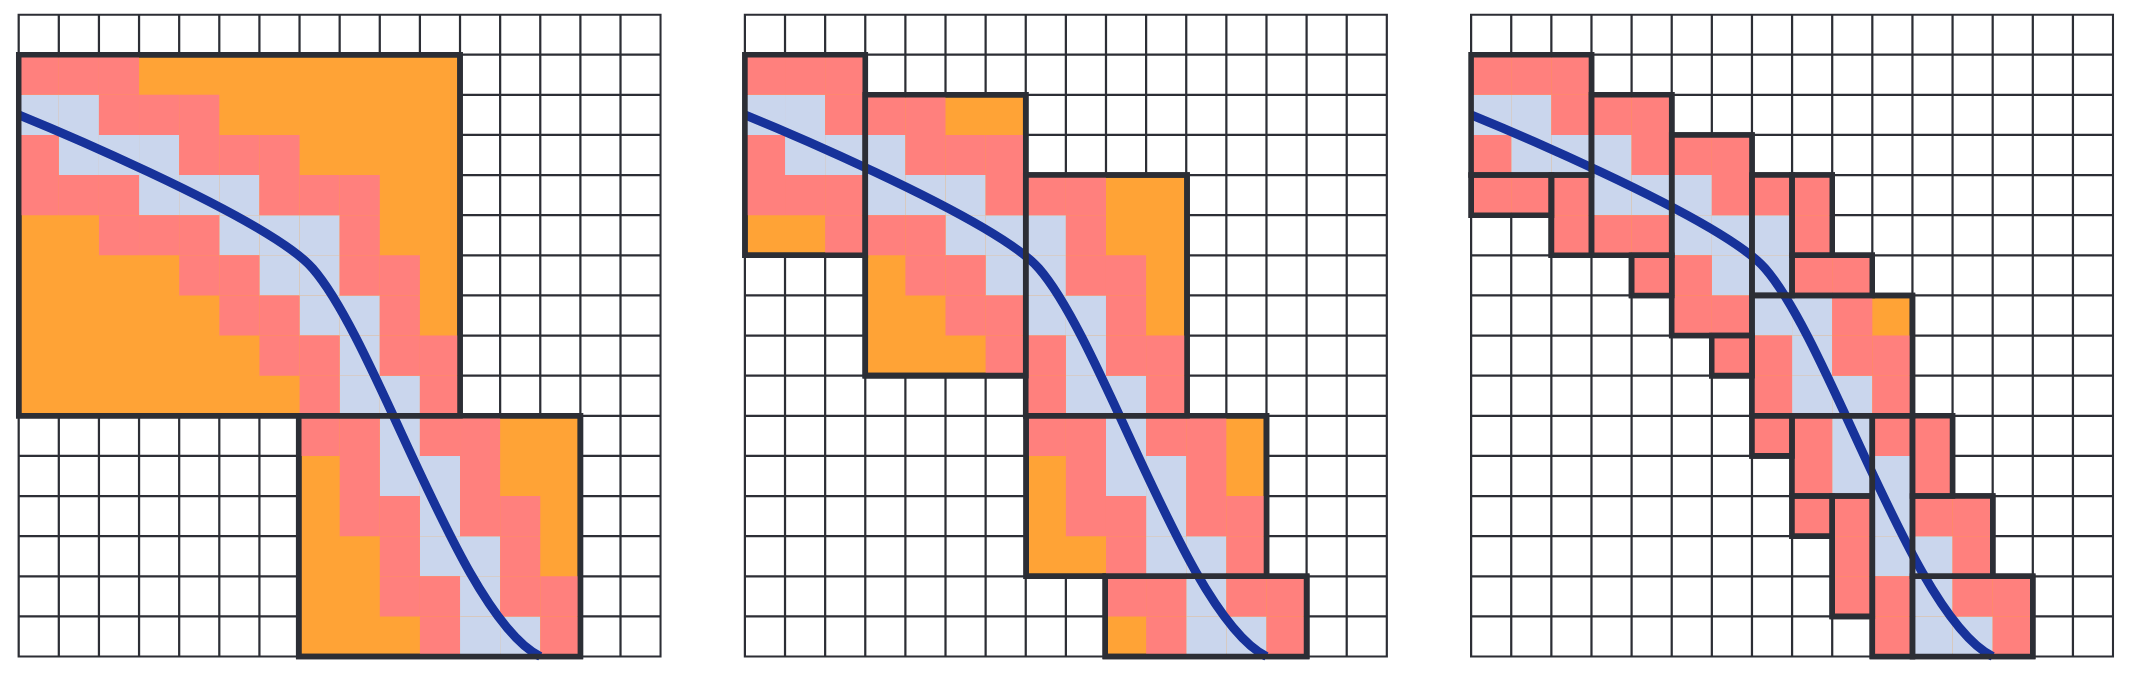
\includegraphics[scale=0.18]{filling.png}
    \end{figure}
\end{frame}

\section{Multiresolution}

\begin{frame}{Multiresolution Representation}
    \begin{itemize}
        \item<1->``The goal of a multi-scale decomposition of a discrete set of
            data is a rearrangement of its information content in such a way
            that the new discrete representation, exactly equivalent to the old
            one, is more manageable in some respects." - Arandiga, Donat
        \item<2-> The multiresolution scheme introduced by Harten does
            \textit{not} adapt grid.  Instead, a wavelet decomposition is
            performed on the uniform grid.
    \end{itemize}
\end{frame}

\begin{frame}{Multiresolution Representation}
    Define multiple levels of representation of the discrete data
    \begin{equation*}
        \mathcal{G}^{l} = \left\{ x^{l}_{i+\frac{1}{2}} \right\}_{i=1}^{N_{l}} =
            \left\{ x^{l+1}_{i+\frac{1}{2}} \right\}_{i=1,\text{i even}}^{N_{l+1}}
    \end{equation*}
    \begin{figure}
    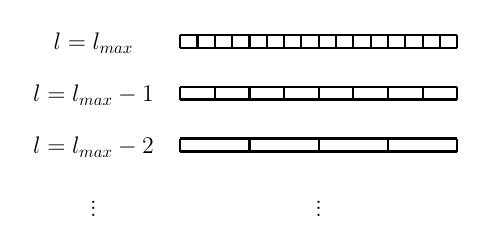
\begin{tikzpicture}[thick,scale=0.22, every node/.style={scale=0.6}]

            % variables
            \def\xl{-8.0}
            \def\xr{8.0}
            \def\y{0.0}
            \def\yy{-3.0}
            \def\yyy{-6.0}
            \def\ts{0.75}
            \def\op{0.35}
            \def\fx{0.15}

            % draw grids
            \draw (\xl,\y) --(\xr,\y);
            \draw (\xl,\y+\ts) --(\xr,\y+\ts);
            \draw (\xl,\yy) --(\xr,\yy);
            \draw (\xl,\yy+\ts) --(\xr,\yy+\ts);
            \draw (\xl,\yyy) --(\xr,\yyy);
            \draw (\xl,\yyy+\ts) --(\xr,\yyy+\ts);

            % draw cells for max level
            \draw (\xl,\y) --(\xl,\y+\ts);
            \draw (\xl+1.0,\y) --(\xl+1.0,\y+\ts);
            \draw (\xl+2.0,\y) --(\xl+2.0,\y+\ts);
            \draw (\xl+3.0,\y) --(\xl+3.0,\y+\ts);
            \draw (\xl+4.0,\y) --(\xl+4.0,\y+\ts);
            \draw (\xl+5.0,\y) --(\xl+5.0,\y+\ts);
            \draw (\xl+6.0,\y) --(\xl+6.0,\y+\ts);
            \draw (\xl+7.0,\y) --(\xl+7.0,\y+\ts);
            \draw (\xl+8.0,\y) --(\xl+8.0,\y+\ts);
            \draw (\xl+9.0,\y) --(\xl+9.0,\y+\ts);
            \draw (\xl+10.0,\y) --(\xl+10.0,\y+\ts);
            \draw (\xl+11.0,\y) --(\xl+11.0,\y+\ts);
            \draw (\xl+12.0,\y) --(\xl+12.0,\y+\ts);
            \draw (\xl+13.0,\y) --(\xl+13.0,\y+\ts);
            \draw (\xl+14.0,\y) --(\xl+14.0,\y+\ts);
            \draw (\xl+15.0,\y) --(\xl+15.0,\y+\ts);
            \draw (\xl+16.0,\y) --(\xl+16.0,\y+\ts);

            % lower level cells
            \draw (\xl,\yy) --(\xl,\yy+\ts);
            \draw (\xl+2.0,\yy) --(\xl+2.0,\yy+\ts);
            \draw (\xl+4.0,\yy) --(\xl+4.0,\yy+\ts);
            \draw (\xl+6.0,\yy) --(\xl+6.0,\yy+\ts);
            \draw (\xl+8.0,\yy) --(\xl+8.0,\yy+\ts);
            \draw (\xl+10.0,\yy) --(\xl+10.0,\yy+\ts);
            \draw (\xl+12.0,\yy) --(\xl+12.0,\yy+\ts);
            \draw (\xl+14.0,\yy) --(\xl+14.0,\yy+\ts);
            \draw (\xl+16.0,\yy) --(\xl+16.0,\yy+\ts);

            % even lower level cells
            \draw (\xl,\yyy) --(\xl,\yyy+\ts);
            \draw (\xl+4.0,\yyy) --(\xl+4.0,\yyy+\ts);
            \draw (\xl+8.0,\yyy) --(\xl+8.0,\yyy+\ts);
            \draw (\xl+12.0,\yyy) --(\xl+12.0,\yyy+\ts);
            \draw (\xl+16.0,\yyy) --(\xl+16.0,\yyy+\ts);

            % nodes
            \node at (\xl-5.0,\y+0.25) {\Large $l=l_{max}$};
            \node at (\xl-5.0,\yy+0.25) {\Large $l=l_{max}-1$};
            \node at (\xl-5.0,\yyy+0.25) {\Large $l=l_{max}-2$};
            \node at (\xl-5.0,\yyy-3.0) {\Large $\vdots$};
            \node at (0,\yyy-3.0) {\Large $\vdots$};

        \end{tikzpicture}
    \end{figure}

\end{frame}

\begin{frame}{Decomposition}
    Coarsening of avarage data in cell done via
    \begin{equation*}
        \mathbf{U}^{l}_{i} = \frac{1}{2} \left( \mathbf{U}^{l+1}_{2i} +
        \mathbf{U}^{l+1}_{2i+1} \right),
    \end{equation*}
    and prediction from coarse to fine is done by
    \begin{equation*}
        \mathbf{\hat{U}}^{l+1}_{2i+1} = \sum_{j=1-s}^{s-1} \gamma_{j}
        \mathbf{U}^{l}_{i+j},
    \end{equation*}
    where $\gamma_{j}$ are average-interpolation coefficients.
\end{frame}

\begin{frame}[shrink=25]{Detail Coefficients}
    The regularity information is assessed by computing detail coefficients
    (residuals) as
    \begin{equation*}
        \mathbf{d}^{l}_{i} = \mathbf{U}^{l+1}_{2i+1} - \mathbf{\hat{U}}^{l+1}_{2i+1}.
    \end{equation*}
    \begin{figure}
        \center
        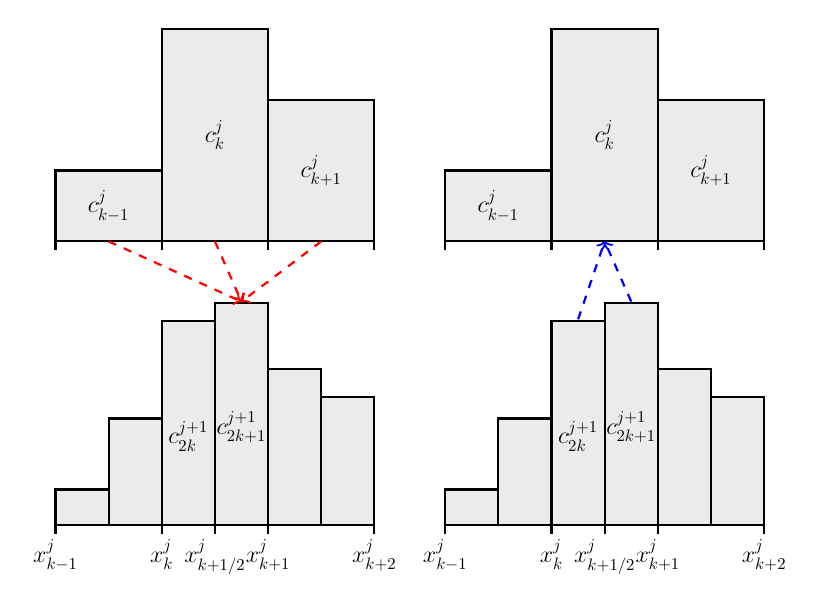
\begin{tikzpicture}[thick,scale=0.45, every node/.style={scale=0.6}]

    % variables
    \def\x{-8.0}
    \def\y{0.0}
    \def\yl{-8.0}
    
    % draw coarse level rectangles
    \draw [fill=mygray] (\x,0) rectangle (\x+3,2);
    \draw [fill=mygray] (\x+3,0) rectangle (\x+6,6);
    \draw [fill=mygray] (\x+6,0) rectangle (\x+9,4);
    
    % coarse level symbols
    \node at (\x+1.5,1) {\Large $c^{j}_{k-1}$};
    \node at (\x+4.5,3) {\Large $c^{j}_{k}$};
    \node at (\x+7.5,2) {\Large $c^{j}_{k+1}$};
    
    % coarse level axis
    \draw (\x,0) -- (\x,-0.25);
    \draw (\x+3,0) -- (\x+3,-0.25);
    \draw (\x+6,0) -- (\x+6,-0.25);
    \draw (\x+9,0) -- (\x+9,-0.25);

    % fine level rectangles
    \draw [fill=mygray] (\x,\yl) rectangle (\x+1.5,\yl+1);
    \draw [fill=mygray] (\x+1.5,\yl) rectangle (\x+3,\yl+3);
    \draw [fill=mygray] (\x+3,\yl) rectangle (\x+4.5,\yl+5.75);
    \draw [fill=mygray] (\x+4.5,\yl) rectangle (\x+6,\yl+6.25);
    \draw [fill=mygray] (\x+6,\yl) rectangle (\x+7.5,\yl+4.4);
    \draw [fill=mygray] (\x+7.5,\yl) rectangle (\x+9,\yl+3.6);
    
    % fine level symbols
    \node at (\x+3.75,\yl+2.5) {\Large $c^{j+1}_{2k}$};
    \node at (\x+5.25,\yl+2.75) {\Large $c^{j+1}_{2k+1}$};
    
    % fine level axis
    \draw (\x,\yl) -- (\x,\yl-0.25);
    \draw (\x+3,\yl) -- (\x+3,\yl-0.25);
    \draw (\x+4.5,\yl) -- (\x+4.5,\yl-0.25);
    \draw (\x+6,\yl) -- (\x+6,\yl-0.25);
    \draw (\x+9,\yl) -- (\x+9,\yl-0.25);

    % arrows
    \draw[red,dashed,->] (\x+1.5,\y) -- (\x+5.25,\y-1.7);
    \draw[red,dashed,->] (\x+4.5,\y) -- (\x+5.25,\y-1.7);
    \draw[red,dashed,->] (\x+7.5,\y) -- (\x+5.25,\y-1.7);

    % tick text
    \node[below] at (\x,\yl-0.25) {\Large $x^{j}_{k-1}$};
    \node[below] at (\x+3,\yl-0.25) {\Large $x^{j}_{k}$};
    \node[below] at (\x+4.5,\yl-0.25) {\Large $x^{j}_{k+1/2}$};
    \node[below] at (\x+6,\yl-0.25) {\Large $x^{j}_{k+1}$};
    \node[below] at (\x+9,\yl-0.25) {\Large $x^{j}_{k+2}$};
    
    %----
    
    % variables
    \def\x{3.0}
    \def\y{0.0}
    \def\yl{-8.0}
    
    % draw coarse level rectangles
    \draw [fill=mygray] (\x,0) rectangle (\x+3,2);
    \draw [fill=mygray] (\x+3,0) rectangle (\x+6,6);
    \draw [fill=mygray] (\x+6,0) rectangle (\x+9,4);
    
    % coarse level symbols
    \node at (\x+1.5,1) {\Large $c^{j}_{k-1}$};
    \node at (\x+4.5,3) {\Large $c^{j}_{k}$};
    \node at (\x+7.5,2) {\Large $c^{j}_{k+1}$};
    
    % coarse level axis
    \draw (\x,0) -- (\x,-0.25);
    \draw (\x+3,0) -- (\x+3,-0.25);
    \draw (\x+6,0) -- (\x+6,-0.25);
    \draw (\x+9,0) -- (\x+9,-0.25);

    % fine level rectangles
    \draw [fill=mygray] (\x,\yl) rectangle (\x+1.5,\yl+1);
    \draw [fill=mygray] (\x+1.5,\yl) rectangle (\x+3,\yl+3);
    \draw [fill=mygray] (\x+3,\yl) rectangle (\x+4.5,\yl+5.75);
    \draw [fill=mygray] (\x+4.5,\yl) rectangle (\x+6,\yl+6.25);
    \draw [fill=mygray] (\x+6,\yl) rectangle (\x+7.5,\yl+4.4);
    \draw [fill=mygray] (\x+7.5,\yl) rectangle (\x+9,\yl+3.6);
    
    % fine level symbols
    \node at (\x+3.75,\yl+2.5) {\Large $c^{j+1}_{2k}$};
    \node at (\x+5.25,\yl+2.75) {\Large $c^{j+1}_{2k+1}$};
    
    % fine level axis
    \draw (\x,\yl) -- (\x,\yl-0.25);
    \draw (\x+3,\yl) -- (\x+3,\yl-0.25);
    \draw (\x+4.5,\yl) -- (\x+4.5,\yl-0.25);
    \draw (\x+6,\yl) -- (\x+6,\yl-0.25);
    \draw (\x+9,\yl) -- (\x+9,\yl-0.25);

    % arrows
    \draw[blue,dashed,->] (\x+5.25,\y-1.7) -- (\x+4.5,\y);
    \draw[blue,dashed,->] (\x+3.75,\y-2.2) -- (\x+4.5,\y);

    % tick text
    \node[below] at (\x,\yl-0.25) {\Large $x^{j}_{k-1}$};
    \node[below] at (\x+3,\yl-0.25) {\Large $x^{j}_{k}$};
    \node[below] at (\x+4.5,\yl-0.25) {\Large $x^{j}_{k+1/2}$};
    \node[below] at (\x+6,\yl-0.25) {\Large $x^{j}_{k+1}$};
    \node[below] at (\x+9,\yl-0.25) {\Large $x^{j}_{k+2}$};
    
\end{tikzpicture}

    \end{figure}
\end{frame}

\begin{frame}{Multiresolution Representation}
    \begin{figure}
        \center
        \includegraphics[scale=0.45]{eps0.png}
    \end{figure}
\end{frame}

\begin{frame}{Multiresolution Representation}
    \begin{figure}
        \center
        \includegraphics[scale=0.45]{eps1e6.png}
    \end{figure}
\end{frame}

\begin{frame}{Multiresolution Representation}
    \begin{figure}
        \center
        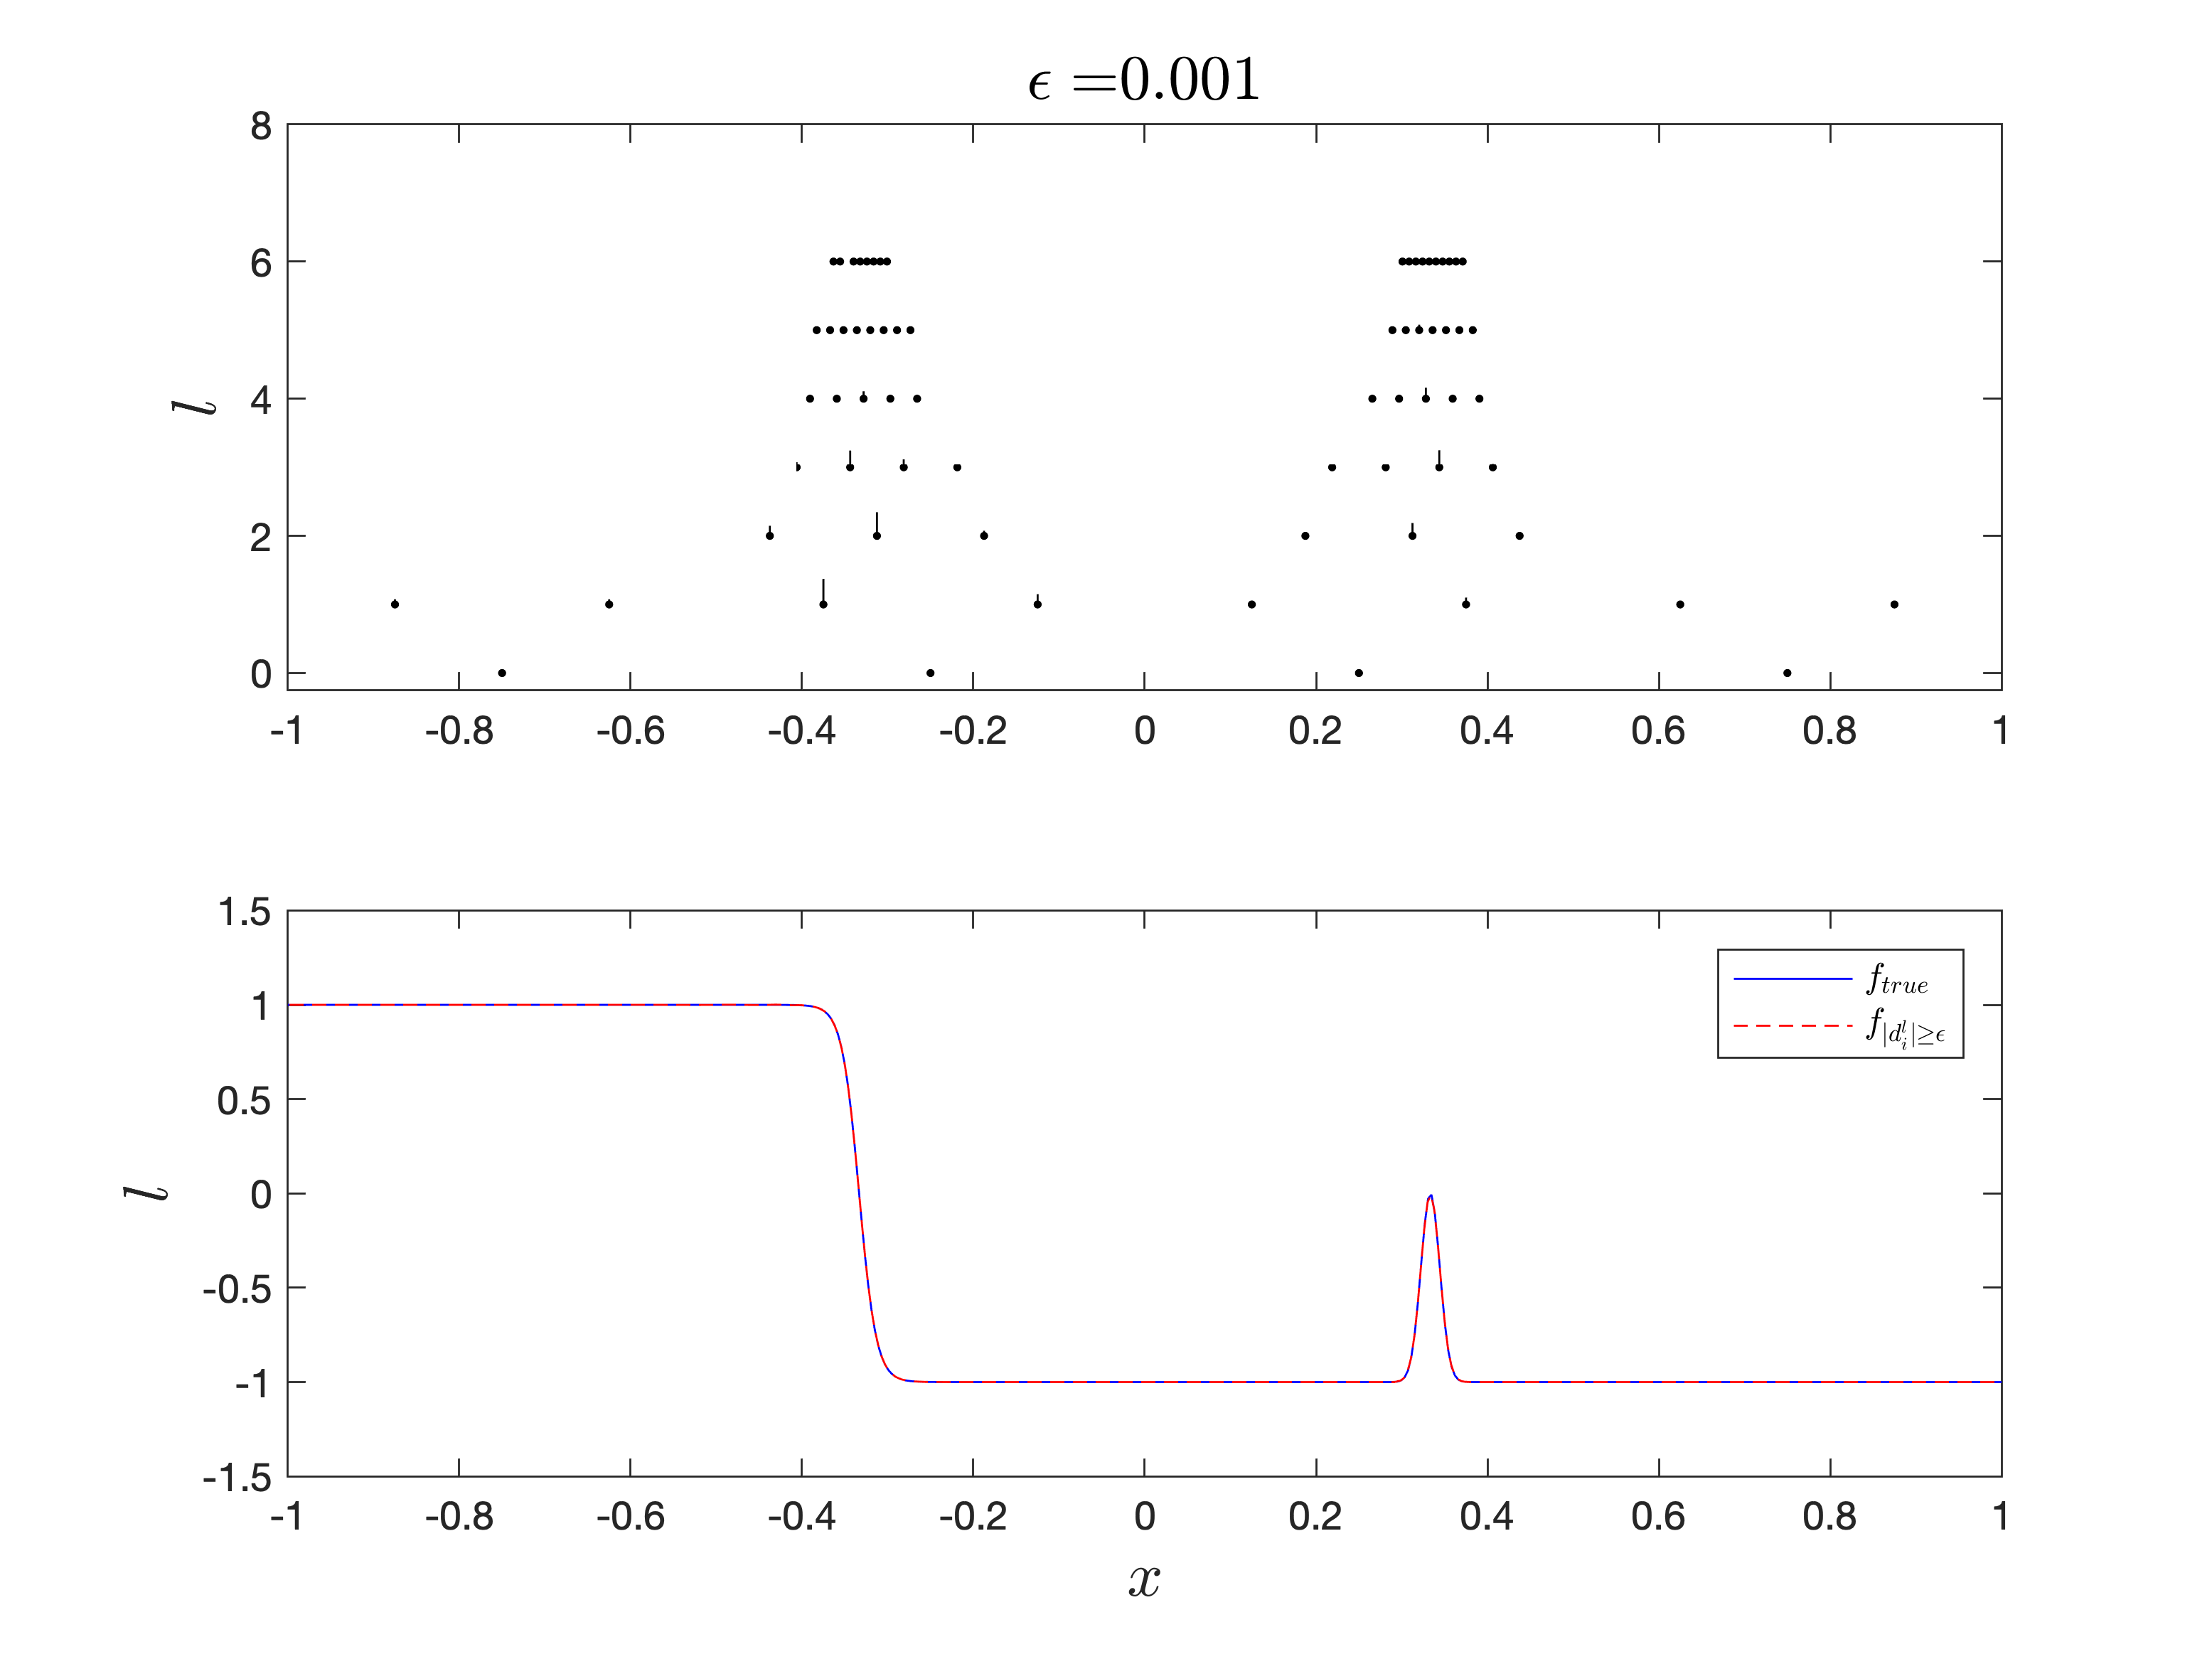
\includegraphics[scale=0.45]{eps1e3.png}
    \end{figure}
\end{frame}

\begin{frame}{Multiresolution Representation}
    \begin{figure}
        \center
        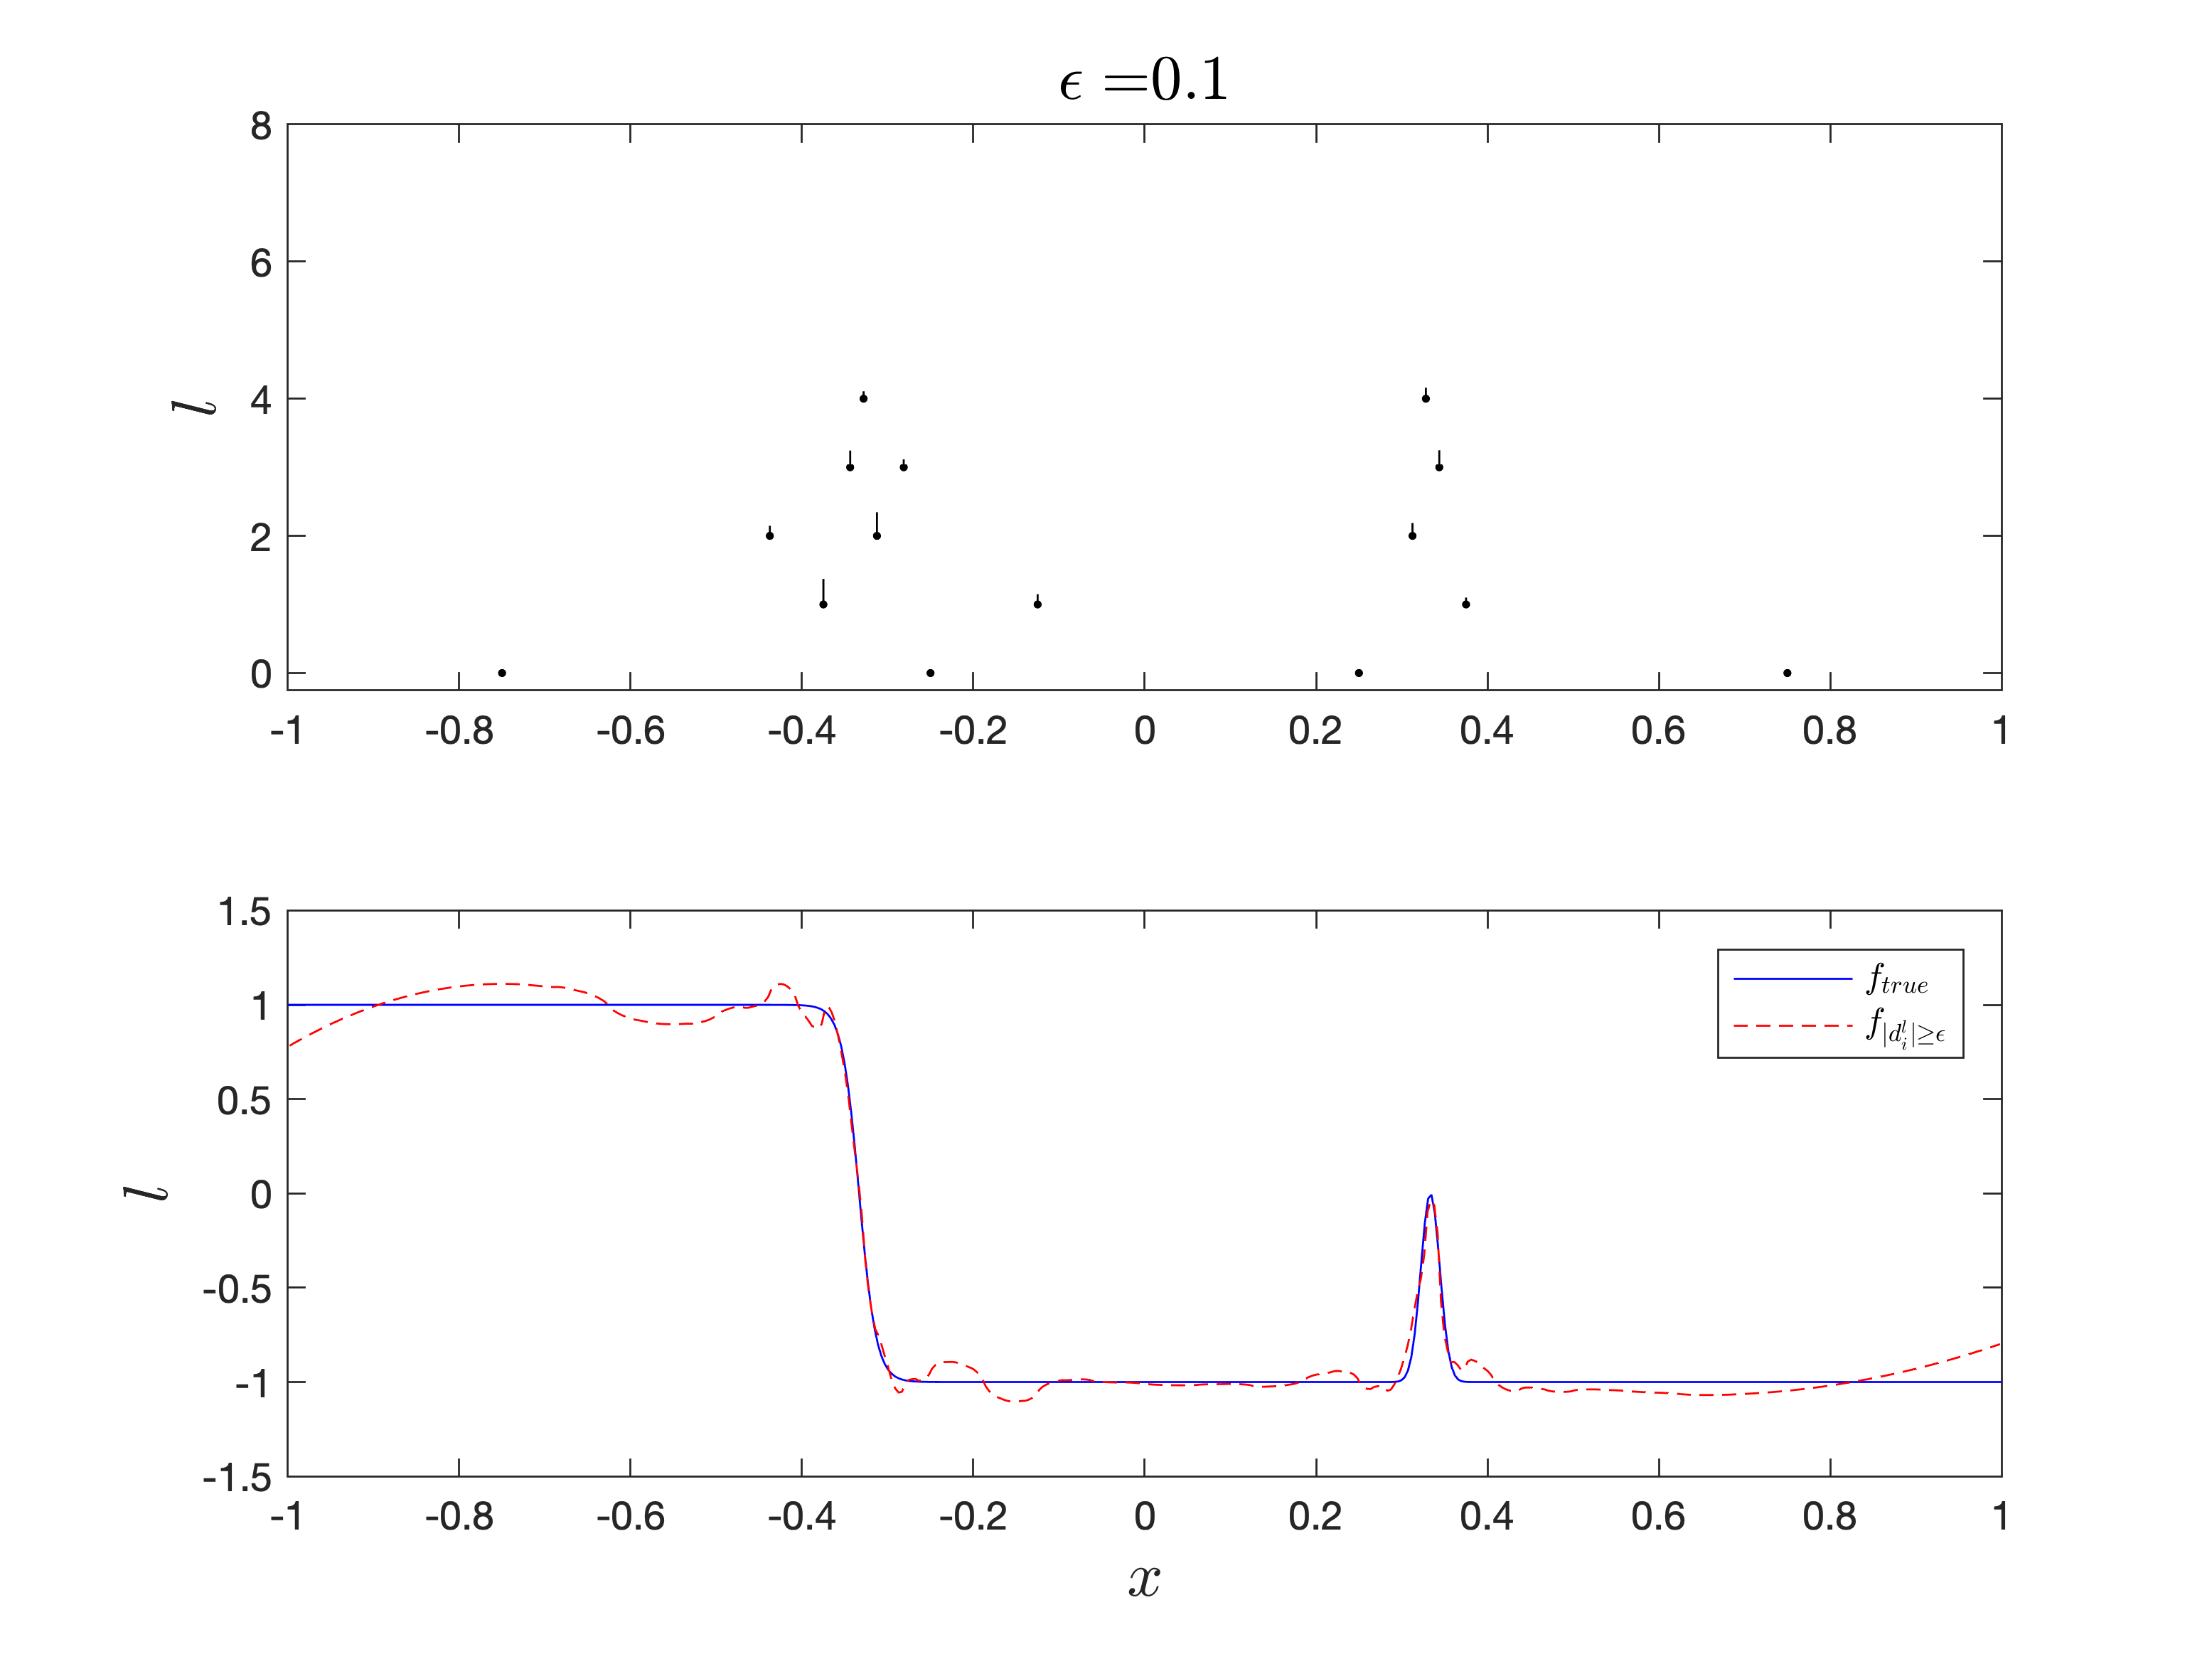
\includegraphics[scale=0.45]{eps1e1.png}
    \end{figure}
\end{frame}

\begin{frame}{Harten's Approach}
    \begin{equation*}
        \frac{\partial \mathbf{U}_{i}}{\partial t} = -\frac{1}{|V_{i}|} \left( \mathbf{F}_{i+\frac{1}{2}}
            - \mathbf{F}_{i-\frac{1}{2}} \right) + \mathbf{S}_{i}
    \end{equation*}
    \begin{itemize}
        \item<2-> compute multiresolution decomposition on solution data
        \item<2-> utilize this regularity information to identify smooth regions
        \item<3-> move from coarse to fine, either compute or interpolate each
            $F^{l}_{i\pm \frac{1}{2}}$
    \end{itemize}
\end{frame}

\begin{frame}{Convergence}
  Sine wave advection after one period:
  \begin{figure}
    \center
    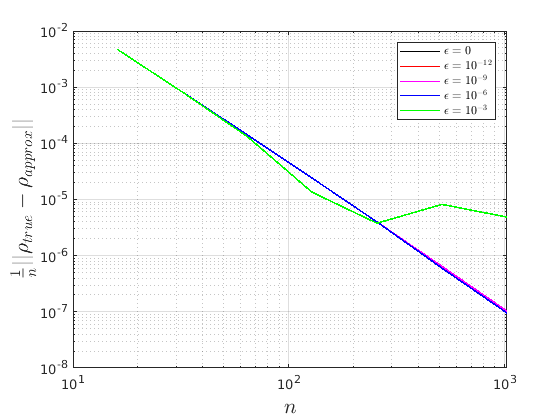
\includegraphics[scale=0.5]{convergence.png}
  \end{figure}
\end{frame}

\begin{frame}{Two Interacting Blast Waves}
  \begin{figure}
    \center
    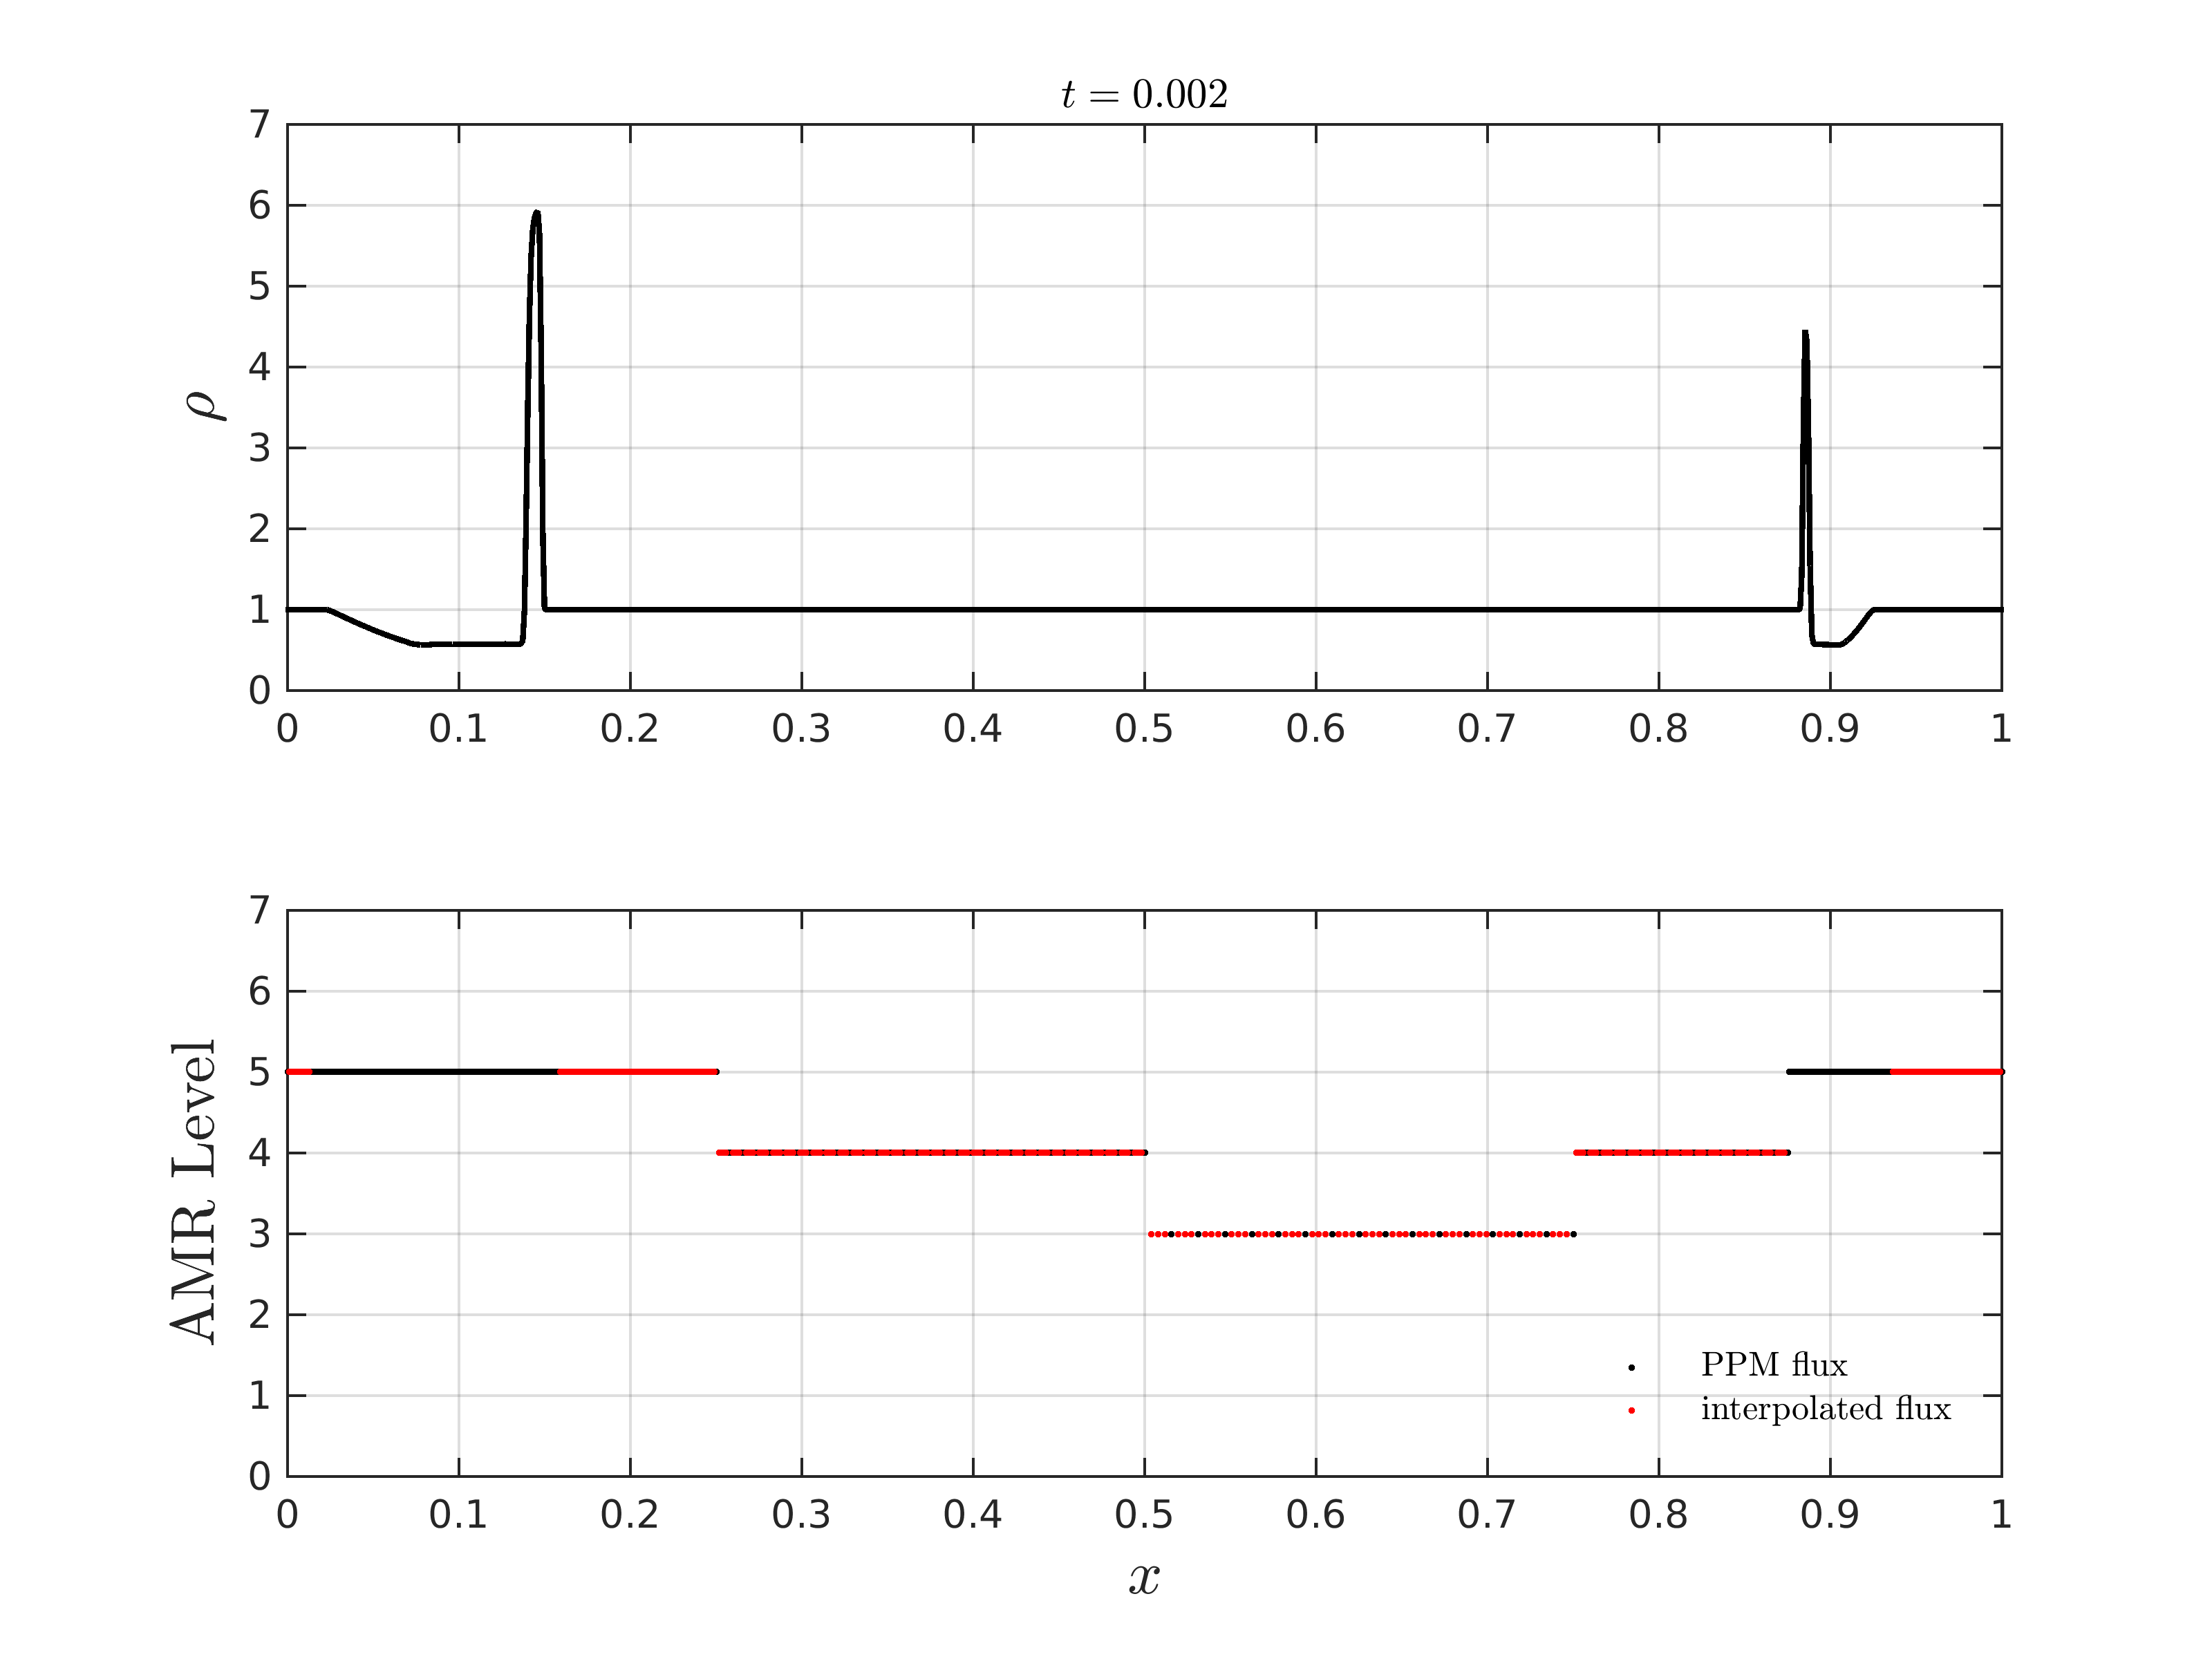
\includegraphics[scale=0.4]{blast2_early.png}
  \end{figure}
\end{frame}

\begin{frame}{Two Interacting Blast Waves}
  \begin{figure}
    \center
    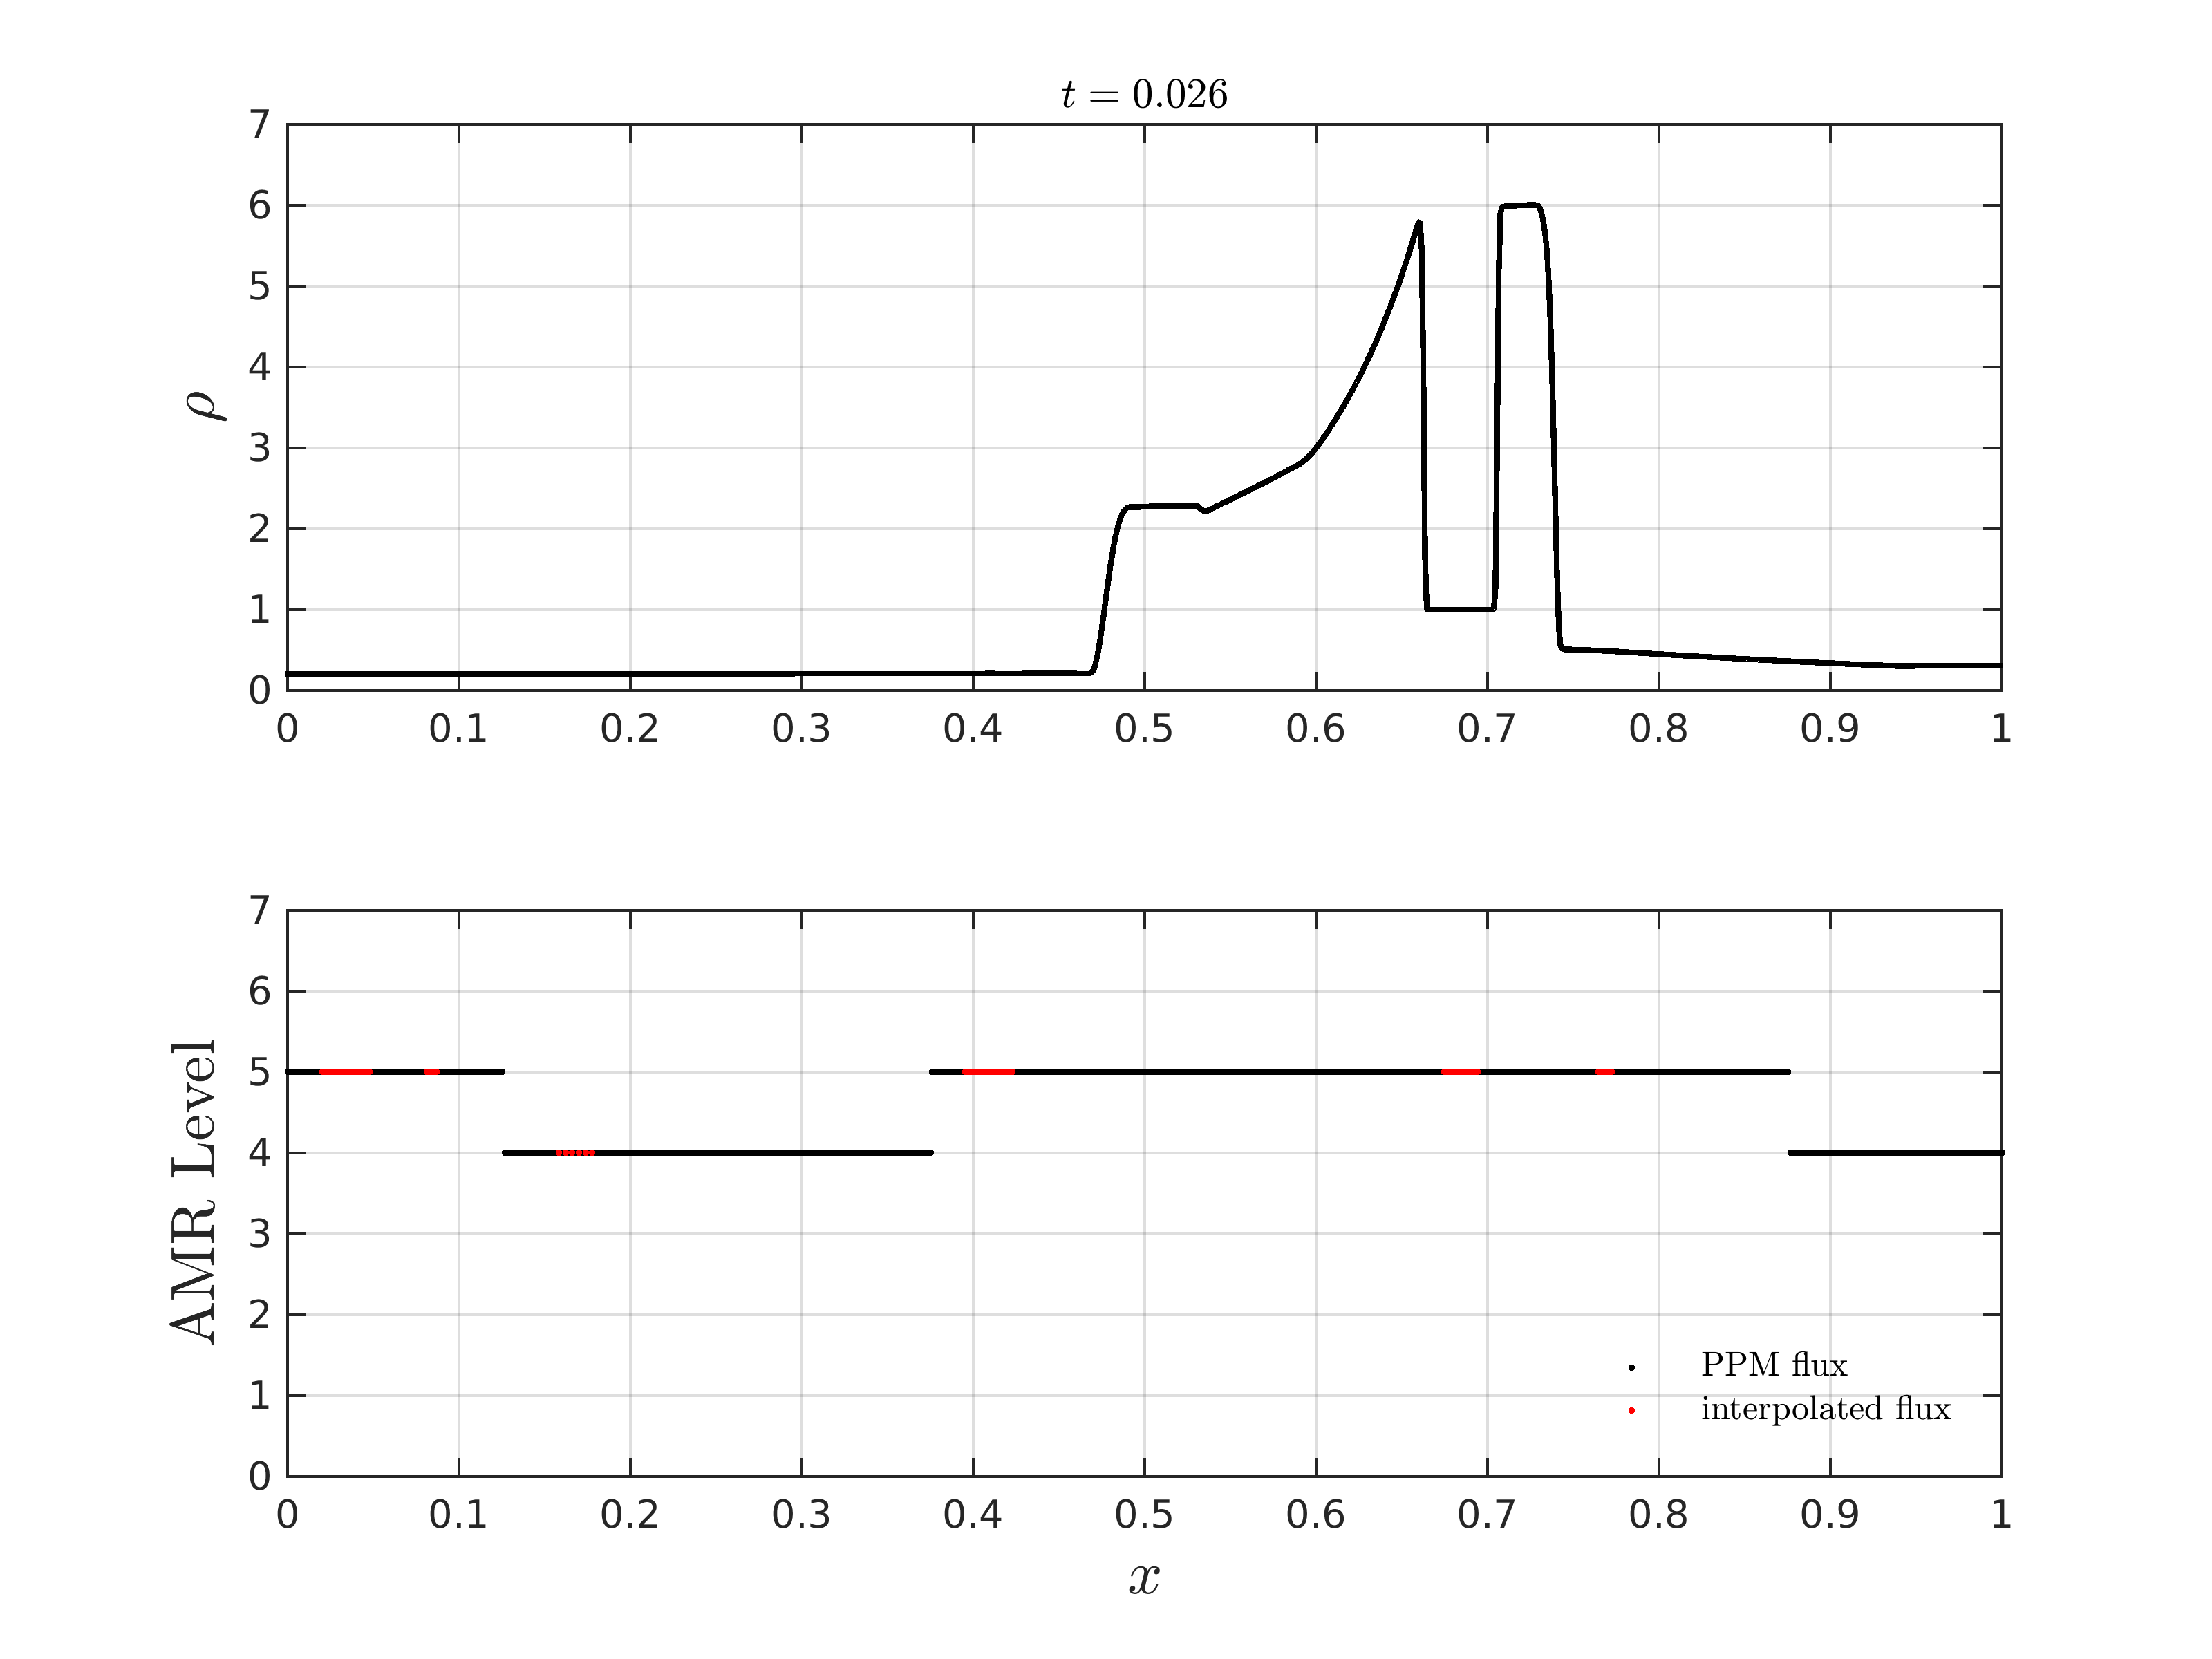
\includegraphics[scale=0.4]{blast2_late.png}
  \end{figure}
\end{frame}

\begin{frame}{Two Interacting Blast Waves}
  \begin{figure}
    \center
    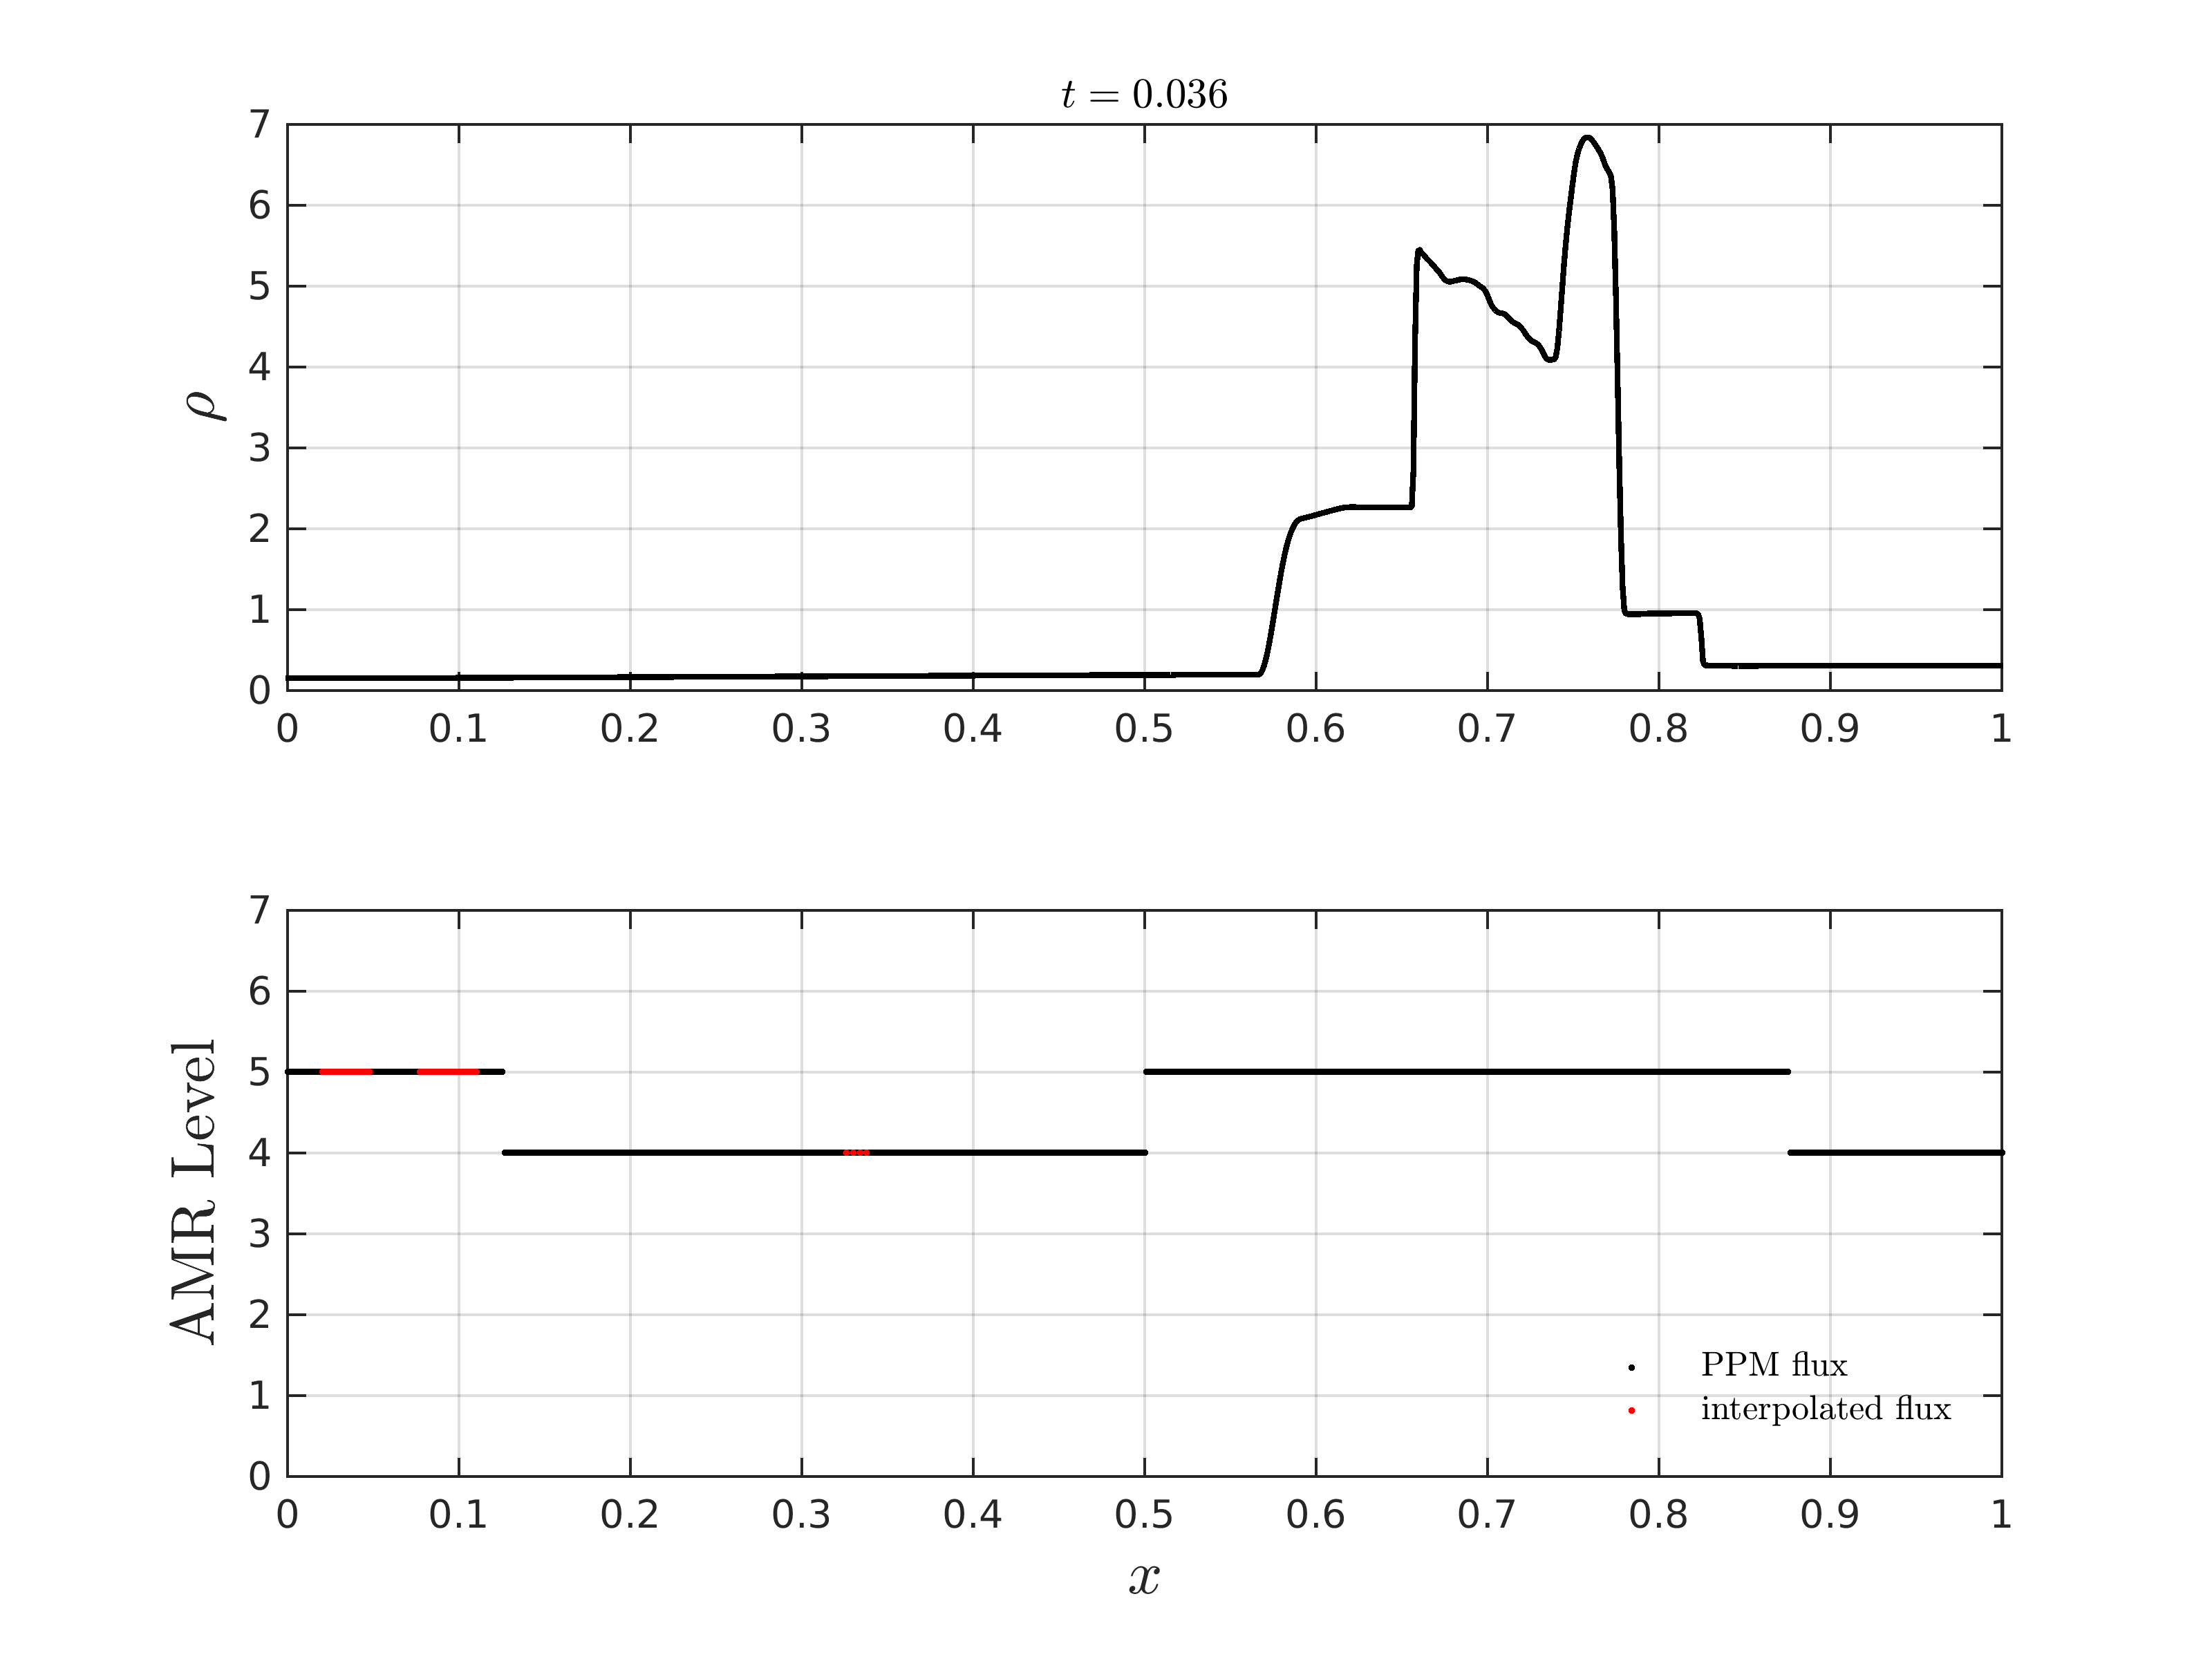
\includegraphics[scale=0.4]{blast2_vlate.png}
  \end{figure}
\end{frame}

\begin{frame}{Future}
    \begin{itemize}
        \item<1-> analyze efficiency of the approach
        \item<2-> move to multi-dimensional problems
    \end{itemize}
\end{frame}

\end{document}
